\documentclass[%
 reprint,
 amsmath,amssymb,
 aps,
 floatfix,
]{revtex4-2}

\usepackage{graphicx}
\graphicspath{{figures/}}
\usepackage{bm}
\usepackage[colorlinks=true,linkcolor=blue,citecolor=blue,urlcolor=blue]{hyperref}
% Wrapper for the sentences that cite the background figures.
\newcommand{\revtexonly}[1]{#1}

\begin{document}

\title{Quantum states of light in cavity QED: A computational study of Wigner function dynamics and atom--field entanglement in the Jaynes--Cummings model}

\author{Nguyen Khoi Nguyen}
\affiliation{Department of Electrical and Computer Engineering, Boston University, Boston, Massachusetts 02215, USA}
\affiliation{Department of Physics, Boston University, Boston, Massachusetts 02215, USA}

\date{\today}

\begin{abstract}
We study numerically the resonant Jaynes--Cummings (JC) model for an initially excited two-level atom coupled with strength $g$ to a cavity field of mean photon number $\bar{n} = 10$, with and without cavity loss, after a self-contained derivation of the model and of its collapse and revival times. Time-resolved Wigner functions show a coherent field evolving into a Schr\"{o}dinger-cat-like state at half the revival time, with Wigner negativity $\delta = 0.85$, purity $0.96$, and fidelity $0.78$ with a two-component cat state. At that time the atom and field approximately disentangle (reduced atomic entropy $S \approx 0.14$~bit), so that the field alone is in a nearly pure state. Comparing coherent, thermal, squeezed-vacuum, and Fock initial fields through the reduced atomic entropy and the logarithmic negativity, we find this disentanglement only for the coherent field; for the thermal field the entropy saturates near 1~bit while the logarithmic negativity stays near 0.2, which shows that the reduced entropy is not an entanglement measure once the global state is mixed. A cavity decay rate $\kappa = 0.02\,g$ already reduces the Wigner negativity at half the revival time by more than 80\%.
\end{abstract}

\keywords{quantum optics, Jaynes--Cummings model, Wigner function, entanglement entropy, cavity QED, Schr\"{o}dinger cat state, decoherence}

\maketitle

%% ============================================================
%% SECTION 1: INTRODUCTION
%% ============================================================
\section{Introduction}
\label{sec:intro}

Coherent manipulation of quantum two-level systems underlies most schemes for controlling qubits. Rabi oscillations, the periodic cycling of population between two quantum states under a resonant driving field~\cite{rabi1937}, provide the physical mechanism~\cite{scully1997}. When a two-level system is driven on resonance, its state oscillates between the ground and excited states at the Rabi frequency, which is set by the coupling strength to the field~\cite{allen1975, gerry2004}. By choosing the duration and phase of the driving pulse, one can prepare arbitrary superpositions or implement state flips, the operations on which quantum gates are built.

The Jaynes--Cummings (JC) model~\cite{jaynes1963}, which describes the interaction of a single two-level atom with a single quantized cavity mode, is the simplest fully quantum model of light--matter interaction. It predicts the vacuum Rabi splitting and, with no classical analog, the collapse and revival of Rabi oscillations~\cite{eberly1980} and the dynamical generation of Schr\"{o}dinger cat states of the cavity field~\cite{gea-banacloche1990, gea-banacloche1991}. These predictions have been tested in cavity quantum electrodynamics (QED) experiments with Rydberg atoms in microwave cavities~\cite{rempe1987, brune1996rabi, auffeves2003, haroche2006} and, more recently, in circuit QED with superconducting qubits coupled to microwave resonators~\cite{blais2021}.

Textbook treatments of the JC model emphasize the collapse and revival of the atomic inversion; the accompanying phase-space dynamics of the field and the atom--field entanglement, analyzed in Refs.~\cite{gea-banacloche1990, gea-banacloche1991, phoenix1988, phoenix1991}, are less often presented together. In this paper we combine a self-contained theoretical introduction with numerical simulations that address three points. First, we compute the time-resolved Wigner function of the cavity field during JC dynamics, which shows the formation and destruction of cat states in phase space, and we quantify their nonclassicality by the Wigner negativity. Second, we compare the atom--field entanglement for four classes of initial field states (coherent, thermal, squeezed vacuum, and Fock), using the reduced atomic entropy where the global state is pure and the logarithmic negativity where it is mixed; the comparison shows how the photon statistics of the field govern the entanglement dynamics and, in particular, that among these fields the atom and field approximately disentangle at half the revival time only for a coherent field. Third, we include cavity dissipation through the Lindblad master equation and quantify how rapidly decoherence destroys the nonclassical features.

The paper is organized as follows. Section~\ref{sec:theory} reviews the quantization of the electromagnetic field, the principal quantum states of light, and the Wigner function; derives the JC Hamiltonian from the electric-dipole interaction, including the rotating-wave approximation; solves for the dressed states and their limiting behavior; derives the collapse and revival timescales; and introduces the master equation and the entanglement measures used later. Section~\ref{sec:methods} describes the computational methods. Section~\ref{sec:results} presents the simulation results. Section~\ref{sec:criteria} summarizes criteria for nonclassical light. Section~\ref{sec:experiment} relates the results to experiments on four platforms. Section~\ref{sec:conclusions} concludes.


%% ============================================================
%% SECTION 2: THEORETICAL FRAMEWORK
%% ============================================================
\section{Theoretical Framework}
\label{sec:theory}

\subsection{Quantum harmonic oscillator and field quantization}
\label{sec:quantization}

The quantization of the harmonic oscillator is the starting point of quantum optics, since each mode of the electromagnetic field can be treated as a harmonic oscillator. Classically, a harmonic oscillator of mass $m$ and angular frequency $\omega$ has the Hamiltonian $H = p^2/(2m) + \tfrac{1}{2}m\omega^2 x^2$. In quantum mechanics, we promote $x$ and $p$ to operators satisfying $[\hat{x}, \hat{p}] = i\hbar$ and introduce the ladder operator
\begin{equation}
a = \sqrt{\frac{m\omega}{2\hbar}} \left( \hat{x} + \frac{i\hat{p}}{m\omega} \right)
\label{eq:ladder}
\end{equation}
and its adjoint $a^\dagger$, which satisfy $[a, a^\dagger] = 1$. The Hamiltonian becomes $H = \hbar\omega(a^\dagger a + \tfrac{1}{2})$, and the number operator $\hat{n} = a^\dagger a$ has eigenstates $|n\rangle$ (Fock states) with $n = 0, 1, 2, \ldots$. The ladder operators act as $a^\dagger|n\rangle = \sqrt{n+1}\,|n+1\rangle$ and $a|n\rangle = \sqrt{n}\,|n-1\rangle$, giving the quantized energy spectrum $E_n = \hbar\omega(n + \tfrac{1}{2})$ with equally spaced levels separated by $\hbar\omega$. The ground state $|0\rangle$ carries the zero-point energy $\tfrac{1}{2}\hbar\omega$, reflecting irreducible vacuum fluctuations.

To describe light quantum mechanically, we expand the electromagnetic field in a complete set of modes (plane waves or cavity standing waves). Each mode of frequency $\omega_k$ becomes a quantum harmonic oscillator with operators $a_k$ and $a_k^\dagger$. The electric field operator for a single mode takes the form
\begin{equation}
\hat{E}(t) = i\, \mathcal{E}_0 \left( a_k e^{-i \omega_k t} - a_k^\dagger e^{i \omega_k t} \right),
\label{eq:efield}
\end{equation}
where $\mathcal{E}_0 = \sqrt{\hbar \omega_k / (2 \varepsilon_0 V)}$ is the single-photon field amplitude and $V$ is the quantization volume. The operator $a_k$ annihilates one photon in mode $k$, while $a_k^\dagger$ creates one. The total field Hamiltonian is
\begin{equation}
H_{\text{field}} = \sum_k \hbar \omega_k \left( a_k^\dagger a_k + \frac{1}{2} \right).
\label{eq:Hfield}
\end{equation}
The vacuum state has zero-point energy $\tfrac{1}{2} \sum_k \hbar \omega_k$, and excitations are described by multimode Fock states $|n_1, n_2, \ldots\rangle$ specifying the photon count in each mode.


\subsection{Quantum states of light}
\label{sec:states}

\textit{Fock states} $|n\rangle$ are eigenstates of the photon-number operator with a definite number of photons. They have no classical analog: a classical field cannot have an exact integer photon count. Fock states exhibit the quantum granularity of the field; for example, a single-photon state $|1\rangle$ produces at most one detection event, and the vacuum $|0\rangle$ produces none.

\textit{Coherent states} $|\alpha\rangle$, for complex amplitude $\alpha$, play a central role in quantum optics. They are defined as eigenstates of the annihilation operator, $a|\alpha\rangle = \alpha|\alpha\rangle$, or equivalently as displaced vacuum states $|\alpha\rangle = D(\alpha)|0\rangle$ with displacement operator $D(\alpha) = \exp(\alpha a^\dagger - \alpha^* a)$. Expanding in the Fock basis yields a Poissonian photon-number distribution:
\begin{equation}
p(n) = |\langle n|\alpha\rangle|^2 = e^{-|\alpha|^2} \frac{|\alpha|^{2n}}{n!},
\label{eq:poisson}
\end{equation}
with mean $\bar{n} = |\alpha|^2$ and variance $\mathrm{Var}(n) = \bar{n}$. The equality of variance and mean is characteristic of shot-noise-limited light. Coherent states saturate the Heisenberg uncertainty relation for the field quadratures, with equal, vacuum-level noise in both. They are often called the ``most classical'' quantum states because their mean electric field follows a classical sinusoid and their Glauber--Sudarshan $P$ function is a delta function, $P(\beta) = \delta^2(\beta - \alpha)$~\cite{glauber1963, sudarshan1963}. Laser light above threshold is well described by a coherent state with large $\bar{n}$.

\textit{Squeezed states} are nonclassical states in which the quantum noise in one field quadrature is reduced below the vacuum level, at the expense of increased noise in the conjugate quadrature. For the quadrature $X_\vartheta = \tfrac{1}{2}(a e^{-i\vartheta} + a^\dagger e^{i\vartheta})$, the vacuum and every coherent state have the variance $\mathrm{Var}(X_\vartheta) = 1/4$ for all $\vartheta$. A squeezed state has $\mathrm{Var}(X_{\vartheta_0}) < 1/4$ for some phase $\vartheta_0$. The squeeze operator $S(\zeta) = \exp[\tfrac{1}{2}(\zeta^* a^2 - \zeta a^{\dagger 2})]$, with $\zeta = r e^{i\phi}$, applied to the vacuum gives the quadrature variances
\begin{equation}
\mathrm{Var}(X_{\phi/2}) = \tfrac{1}{4} e^{-2r}, \quad
\mathrm{Var}(X_{\phi/2 + \pi/2}) = \tfrac{1}{4} e^{2r}.
\label{eq:squeeze}
\end{equation}
Squeezed states can be produced by parametric down-conversion or four-wave mixing. Because they exhibit noise below the vacuum level in one observable, they have no classical description (their $P$ function involves derivatives of delta functions). After a proof-of-principle test on an initial LIGO detector~\cite{aasi2013}, squeezed vacuum has been injected routinely into the Advanced LIGO~\cite{tse2019} and Advanced Virgo~\cite{acernese2019} gravitational-wave detectors since the start of their third observing run in April 2019.


\subsection{Phase-space representations: The Wigner function}
\label{sec:wigner}

The Wigner function provides a quasiprobability distribution in phase space that is particularly useful for visualizing quantum states and identifying nonclassical features. For a single-mode field with density operator $\rho$, it is defined as~\cite{wigner1932}
\begin{equation}
W(x, p) = \frac{1}{\pi\hbar} \int_{-\infty}^{\infty} \langle x - y | \rho | x + y \rangle \, e^{2ipy/\hbar} \, dy,
\label{eq:wigner_def}
\end{equation}
where $x$ and $p$ are conjugate phase-space quadratures. From here on we set $\hbar = 1$ and use the dimensionless quadratures defined by $a = (x + ip)/\sqrt{2}$, that is, $x = \sqrt{2}\,X_0$ and $p = \sqrt{2}\,X_{\pi/2}$, for which the vacuum variances are $1/2$. Unlike a true probability distribution, $W(x,p)$ can take negative values; such negative regions are a sufficient (though not necessary) indicator of nonclassicality~\cite{kenfack2004}, and among pure states only Gaussian states have a nonnegative Wigner function~\cite{hudson1974}.

\begin{figure*}[t]
    \centering
    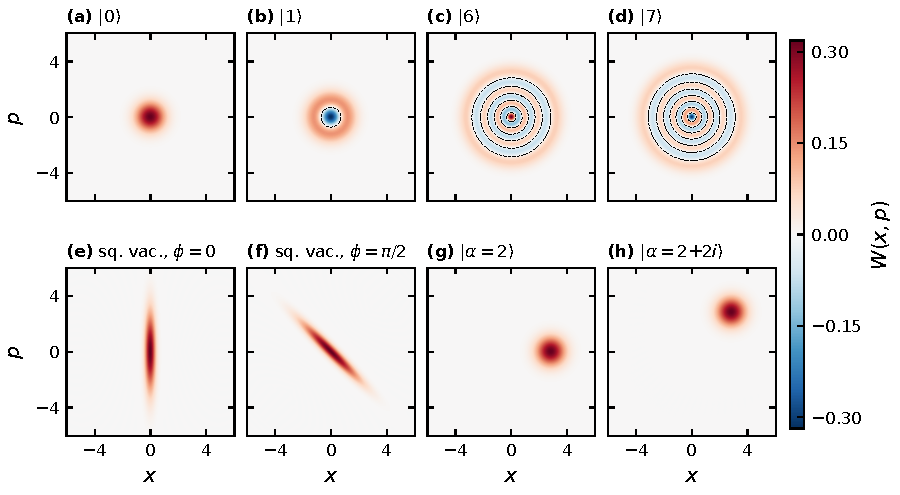
\includegraphics[width=6in]{wigner_functions_2d.pdf}
    \caption{Wigner functions $W(x,p)$ of (a)--(d) the Fock states $|0\rangle$, $|1\rangle$, $|6\rangle$, and $|7\rangle$; (e), (f) the squeezed vacuum with $r = 1$ and $\phi = 0$, $\pi/2$; and (g), (h) the coherent states $|\alpha\rangle$ with $\alpha = 2$ and $2+2i$, on a common color scale in the convention $a = (x + ip)/\sqrt{2}$. Dashed contours mark $W = 0$. Fock states show rings of alternating sign, with $W(0,0) = (-1)^n/\pi$; the squeezed vacuum is an ellipse whose narrow axis lies at the angle $\phi/2$; coherent states are displaced Gaussians.}
    \label{fig:wigner_2d_quantum_states}
\end{figure*}

For a coherent state $|\alpha\rangle$, the Wigner function is a Gaussian centered at $(x_0, p_0) = (\sqrt{2}\,\mathrm{Re}\,\alpha,\, \sqrt{2}\,\mathrm{Im}\,\alpha)$:
\begin{equation}
W_\alpha(x,p) = \frac{1}{\pi} \exp\!\big[-(x - x_0)^2 - (p - p_0)^2\big],
\label{eq:wigner_coherent}
\end{equation}
which is everywhere nonnegative. For a Fock state $|n\rangle$,
\begin{equation}
W_n(x,p) = \frac{(-1)^n}{\pi} \, L_n\!\big(2(x^2 + p^2)\big) \, e^{-(x^2 + p^2)},
\label{eq:wigner_fock}
\end{equation}
where $L_n$ is the $n$th Laguerre polynomial; for $n \geq 1$ this exhibits pronounced negative regions. A squeezed vacuum has an elliptical Gaussian Wigner function with $1/e$ half-widths $e^{-r}$ and $e^{r}$ along the squeezed and antisqueezed quadratures; it remains nonnegative, though its $P$ function is singular.\revtexonly{ Figure~\ref{fig:wigner_2d_quantum_states} shows these Wigner functions on a common color scale.}

A quantitative measure of nonclassicality is the Wigner negativity volume~\cite{kenfack2004}, hereafter the Wigner negativity:
\begin{equation}
\delta = \int \big|W(x,p)\big| \, dx\, dp - 1.
\label{eq:negativity}
\end{equation}
Since $\int W\,dx\,dp = 1$, $\delta$ equals twice the integrated volume of the negative part of $W$. Every state with a nonnegative Wigner function has $\delta = 0$; this includes all classical states but also, for example, the squeezed vacuum, so $\delta > 0$ is a sufficient but not a necessary witness of nonclassicality. We use $\delta$ as a quantitative probe throughout the simulations in Sec.~\ref{sec:results}.


\subsection{Derivation of the Jaynes--Cummings Hamiltonian}
\label{sec:jcm}

We derive the JC model~\cite{jaynes1963} from the electric-dipole form of the light--matter interaction. This is the dipole-gauge counterpart of the minimal-coupling Hamiltonian $(\bm{p} - q\bm{A})^2/(2m)$ for a charge $q$ of mass $m$ in the vector potential $\bm{A}$, to which it is related by a gauge (Power--Zienau--Woolley) transformation~\cite{scully1997}. In the dipole approximation, the interaction between a two-level atom and a single quantized cavity mode of frequency $\omega_c$ is
\begin{equation}
H_{\text{int}} = -\bm{d} \cdot \bm{E},
\end{equation}
where $\bm{d}$ is the atomic dipole operator and $\bm{E} \propto \bm{\varepsilon}(a + a^\dagger)$ is the electric field of the mode at the position of the atom [Eq.~(\ref{eq:efield}) in the Schr\"{o}dinger picture, with the phase of $a$ chosen such that the field is proportional to $a + a^\dagger$], with $\bm{\varepsilon}$ the polarization vector. For two atomic levels $|g\rangle$ and $|e\rangle$ with transition frequency $\omega_a$, the dipole operator is $\bm{d} = \bm{d}_0(\sigma^+ + \sigma^-)$, where $\sigma^+ = |e\rangle\langle g|$, $\sigma^- = |g\rangle\langle e|$, and $\bm{d}_0$ is the transition dipole matrix element. The total Hamiltonian is then
\begin{equation}
H = \hbar\omega_c\, a^\dagger a + \frac{\hbar\omega_a}{2}\sigma_z + \hbar g(\sigma^+ + \sigma^-)(a + a^\dagger),
\label{eq:rabi_full}
\end{equation}
where $\sigma_z = |e\rangle\langle e| - |g\rangle\langle g|$ and the coupling constant $g$ is proportional to $\bm{d}_0 \cdot \bm{\varepsilon}$ and to the single-photon field amplitude $\mathcal{E}_0$. Equation~(\ref{eq:rabi_full}) is the Hamiltonian of the quantum Rabi model. It contains both energy-conserving terms ($a\sigma^+$ and $a^\dagger\sigma^-$) and counter-rotating terms ($a^\dagger\sigma^+$ and $a\sigma^-$) that do not conserve the excitation number.

In the regime $g \ll \omega_a, \omega_c$ and near resonance ($|\omega_a - \omega_c| \ll \omega_a + \omega_c$), the counter-rotating terms oscillate at frequency $\omega_a + \omega_c$ in the interaction picture and average to zero. Dropping them (the rotating-wave approximation) gives the JC Hamiltonian:
\begin{equation}
H_{\text{JC}} = \hbar\omega_c\, a^\dagger a + \frac{\hbar\omega_a}{2}\sigma_z + \hbar g\left(a^\dagger \sigma^- + a\,\sigma^+\right).
\label{eq:HJC}
\end{equation}
The term $a^\dagger\sigma^-$ describes atomic deexcitation with photon emission, and $a\sigma^+$ describes photon absorption with atomic excitation. A symmetry of $H_{\text{JC}}$ is the conservation of the total excitation number $\hat{N} = a^\dagger a + \sigma^+\sigma^-$, which commutes with $H_{\text{JC}}$. The Hilbert space therefore decomposes into the uncoupled ground state $|g, 0\rangle$ and the invariant two-dimensional subspaces $\{|e, n\rangle,\, |g, n{+}1\rangle\}$ with $n = 0, 1, 2, \ldots$, which makes the model exactly solvable.


\subsection{Dressed states and energy eigenvalues}
\label{sec:dressed}

Within the subspace of $n{+}1$ total excitations, the Hamiltonian in the basis $\{|e, n\rangle,\, |g, n{+}1\rangle\}$ reduces, after subtraction of the common energy $(n + \tfrac{1}{2})\hbar\omega_c$, to the $2 \times 2$ matrix
\begin{equation}
H^{(n)} = \frac{\hbar}{2}
\begin{pmatrix}
\Delta & \Omega_0\sqrt{n+1} \\
\Omega_0\sqrt{n+1} & -\Delta
\end{pmatrix},
\label{eq:2x2}
\end{equation}
where $\Delta = \omega_a - \omega_c$ is the detuning and $\Omega_0 = 2g$ is the vacuum Rabi frequency. The coupling matrix element $\langle e, n | H_{\text{JC}} | g, n{+}1\rangle = \hbar g\sqrt{n+1}$ follows from the bosonic commutation relations. The eigenvalues are
\begin{equation}
E_{\pm}(n) = \hbar\omega_c\left(n + \tfrac{1}{2}\right) \pm \frac{\hbar}{2}\,\Omega_n(\Delta),
\label{eq:eigenvalues}
\end{equation}
where the generalized $n$-photon Rabi frequency is
\begin{equation}
\Omega_n(\Delta) = \sqrt{\Delta^2 + \Omega_0^2(n+1)}.
\label{eq:gen_rabi}
\end{equation}
The corresponding eigenstates (dressed states) are
\begin{align}
|n,+\rangle &= \cos(\theta_n/2)\, |e,n\rangle + \sin(\theta_n/2)\, |g,n{+}1\rangle, \label{eq:dressed_plus}\\
|n,-\rangle &= \sin(\theta_n/2)\, |e,n\rangle - \cos(\theta_n/2)\, |g,n{+}1\rangle, \label{eq:dressed_minus}
\end{align}
with the mixing angle $0 \leq \theta_n \leq \pi$ defined by $\cos\theta_n = \Delta/\Omega_n(\Delta)$ and $\sin\theta_n = \Omega_0\sqrt{n+1}/\Omega_n(\Delta)$. These are entangled atom--photon states whose character interpolates between atomlike and photonlike as $\Delta$ is varied. The energy splitting between the two dressed states is $\hbar\Omega_n(\Delta)$.


\subsection{Limiting cases}
\label{sec:limits}

\textit{Resonance} ($\Delta = 0$). The mixing angle is $\theta_n = \pi/2$ and the dressed states become equal superpositions:
\begin{equation}
|n, \pm\rangle = \frac{1}{\sqrt{2}}\left(|e,n\rangle \pm |g,n{+}1\rangle\right).
\end{equation}
The splitting reduces to $\hbar\Omega_0\sqrt{n+1}$. For $n = 0$ (one total excitation), the splitting is $\hbar\Omega_0 = 2\hbar g$, the vacuum Rabi splitting. This is directly analogous to the normal-mode splitting of two coupled oscillators; it was observed spectroscopically with, on average, one atom in an optical cavity~\cite{thompson1992}.

\textit{Large detuning} ($|\Delta| \gg \Omega_0\sqrt{n+1}$). The mixing angle approaches 0 for $\Delta > 0$ and $\pi$ for $\Delta < 0$; in either case the dressed states are only weakly entangled. Expanding $\Omega_n \approx |\Delta| + \Omega_0^2(n+1)/(2|\Delta|)$ gives energy shifts
\begin{equation}
E_\pm(n) \approx \hbar\omega_c\left(n + \tfrac{1}{2}\right) \pm \frac{\hbar}{2}\left(|\Delta| + \frac{\Omega_0^2(n+1)}{2|\Delta|}\right).
\end{equation}
The second-order corrections, proportional to $g^2/\Delta$, are the ac Stark (light) shifts~\cite{haroche2006}. In this regime the eigenstates approach the bare states $|e,n\rangle$ and $|g,n{+}1\rangle$, and the atom--field coupling appears primarily as dispersive frequency shifts rather than coherent population transfer. The transition from resonant Rabi splitting to dispersive shifts as $\Delta$ is varied produces an avoided crossing of width $\hbar\Omega_0\sqrt{n+1}$ at $\Delta = 0$.


\subsection{Rabi oscillations from a Fock-state field}
\label{sec:rabi_fock}

Consider the atom initially excited and the field in a Fock state with $n$ photons: $|\Psi(0)\rangle = |e, n\rangle$. This state is not an eigenstate of the coupled system; it is a superposition of the two dressed states in the $(n{+}1)$-excitation manifold. On resonance,
\begin{equation}
|e, n\rangle = \frac{1}{\sqrt{2}}\left(|n,+\rangle + |n,-\rangle\right).
\end{equation}
Evolving each eigenstate with its eigenphase gives, in the interaction picture (that is, after removing the free evolution $e^{-i\omega_c(n+1/2)t}$ of the manifold),
\begin{equation}
|\Psi(t)\rangle = \cos\!\left(\tfrac{1}{2}\Omega_n t\right)|e,n\rangle - i\sin\!\left(\tfrac{1}{2}\Omega_n t\right)|g,n{+}1\rangle,
\label{eq:rabi_evolution}
\end{equation}
where, on resonance, $\Omega_n \equiv \Omega_n(0) = \Omega_0\sqrt{n+1}$, and the sign of the second term follows from $e^{-iH_{\text{JC}}t/\hbar}$ with the coupling $+\hbar g(a^\dagger\sigma^- + a\sigma^+)$. The excited-state probability oscillates sinusoidally:
\begin{equation}
P_e(t) = \cos^2\!\left(\frac{\Omega_0\sqrt{n+1}}{2}\,t\right),
\label{eq:pe_fock}
\end{equation}
at the $n$-photon Rabi frequency $\Omega_n$. For $n = 0$, this is the vacuum Rabi oscillation: an excited atom in an empty cavity emits and reabsorbs a single photon periodically at frequency $\Omega_0$. For $n \gg 1$, the Rabi frequency $\Omega_0\sqrt{n+1} \approx \Omega_0\sqrt{n}$ is proportional to $\sqrt{n}$, that is, to the classical field amplitude, which is the semiclassical result. These coherent oscillations require the strong-coupling regime, in which $g$ greatly exceeds the cavity and atomic decay rates $\kappa$ and $\gamma$ (Sec.~\ref{sec:lindblad}), so that the photon is not lost during a Rabi cycle~\cite{haroche2006}.


\subsection{Collapse and revival of Rabi oscillations}
\label{sec:collapse_revival}

Now suppose the atom is initially excited and the field is in a coherent state $|\alpha\rangle$ with mean photon number $\bar{n} = |\alpha|^2$, where we take $\alpha$ real and positive. In the Fock basis,
\begin{equation}
|\Psi(0)\rangle = |e\rangle \otimes |\alpha\rangle = e^{-\bar{n}/2}\sum_{n=0}^{\infty} \frac{\alpha^n}{\sqrt{n!}}\,|e, n\rangle,
\end{equation}
and, evolving each Fock component independently via Eq.~(\ref{eq:rabi_evolution}), we obtain the excited-state probability
\begin{equation}
P_e(t) = \sum_{n=0}^{\infty} p(n)\,\cos^2\!\left(\frac{\Omega_0\sqrt{n+1}}{2}\,t\right),
\label{eq:pe_coherent}
\end{equation}
where $p(n) = e^{-\bar{n}}\bar{n}^n/n!$ is the Poisson distribution of Eq.~(\ref{eq:poisson}). Equivalently,
\begin{equation}
P_e(t) = \frac{1}{2} + \frac{1}{2}\sum_{n=0}^{\infty} p(n)\,\cos\!\left(\Omega_0\sqrt{n+1}\,t\right).
\label{eq:pe_cos_sum}
\end{equation}
Equation~(\ref{eq:pe_cos_sum}), like the atomic inversion $\langle\sigma_z\rangle = 2P_e - 1$, is a weighted superposition of cosines at the incommensurate frequencies $\Omega_0\sqrt{n+1}$. The Poisson weights are peaked around $n \approx \bar{n}$ with width $\sqrt{\bar{n}}$, so at short times all components oscillate nearly in phase at the dominant frequency $\Omega_0\sqrt{\bar{n}+1}$.

\textit{Collapse.} As time progresses, the components dephase because neighboring Fock states oscillate at slightly different frequencies. The spread of Rabi frequencies across the Poisson distribution (width $\sigma_n = \sqrt{\bar{n}}$) is
\begin{equation}
\sigma_\Omega \sim \frac{\partial\Omega_n}{\partial n}\bigg|_{\bar{n}} \sigma_n = \frac{\Omega_0}{2\sqrt{\bar{n}}} \sqrt{\bar{n}} = \frac{\Omega_0}{2}.
\end{equation}
The oscillations dephase when $\sigma_\Omega t_c \sim 1$, giving the collapse time
\begin{equation}
t_c \sim \frac{2}{\Omega_0} = \frac{1}{g},
\label{eq:t_collapse}
\end{equation}
independent of $\bar{n}$~\cite{eberly1980}. The numerical prefactor depends on the criterion adopted: linearizing $\sqrt{n+1}$ about $\bar{n}$ and summing Eq.~(\ref{eq:pe_cos_sum}) with the Poisson weights gives $P_e(t) - 1/2 \approx (1/2)\cos(\Omega_0\sqrt{\bar{n}+1}\,t)\,\exp[-g^2t^2\bar{n}/2(\bar{n}+1)]$, an oscillation under a Gaussian envelope that becomes $e^{-g^2t^2/2}$ for $\bar{n} \gg 1$, with $1/e$ time $\sqrt{2}/g$. Throughout this paper we adopt the convention $t_c \equiv 1/g$; for $\bar{n} = 10$ the oscillation amplitude has fallen to 16\% of its initial value at $t = 2t_c$ and to below 2\% at $t = 3t_c$. After the collapse, $P_e(t)$ stays within about $10^{-3}$ of $1/2$ until the revival begins.

\textit{Revival.} Despite the apparent loss of coherence, the oscillations return at a later time. Because the Rabi frequencies $\Omega_0\sqrt{n+1}$ form a discrete set, not a continuum, the phases can realign modulo $2\pi$. To estimate the revival time, we require adjacent Fock components with $n \approx \bar{n}$ to accumulate a phase difference of exactly $2\pi$:
\begin{equation}
\left(\Omega_0\sqrt{\bar{n}+2} - \Omega_0\sqrt{\bar{n}+1}\right) t_r = 2\pi.
\end{equation}
For large $\bar{n}$, $\sqrt{\bar{n}+2} - \sqrt{\bar{n}+1} \approx 1/(2\sqrt{\bar{n}+1})$, giving
\begin{equation}
t_r \approx \frac{4\pi\sqrt{\bar{n}}}{\Omega_0} = \frac{2\pi\sqrt{\bar{n}}}{g}.
\label{eq:t_revival}
\end{equation}
Equation~(\ref{eq:t_revival}) is the leading-order result: the envelope of the first revival peaks at $2\pi\sqrt{\bar{n}+1}/g$, which for $\bar{n} = 10$ is about $1/g$ later. We define $t_r \equiv 2\pi\sqrt{\bar{n}}/g$ and use it as the reference time throughout. The ratio $t_r/t_c = 2\pi\sqrt{\bar{n}}$ shows that for large $\bar{n}$ the revival occurs many collapse times later, with a broad plateau of near-zero oscillation amplitude in between.

The revival is a purely quantum effect. A classical field with a continuous amplitude distribution would produce irreversible dephasing with no recurrence. The revival requires the \textit{discrete} spectrum of Fock-state Rabi frequencies, and its observation constitutes direct evidence that the intracavity field is quantized~\cite{eberly1980, haroche2006}.

The revival is incomplete: for $\bar{n} = 10$ the oscillation amplitude returns to 0.57 of its initial value, and the revival lasts about three times longer than the initial collapse. Further revivals occur near integer multiples of $t_r$, each weaker and broader than the one before, until successive revivals overlap~\cite{gerry2004}.

\begin{figure*}[t]
    \centering
    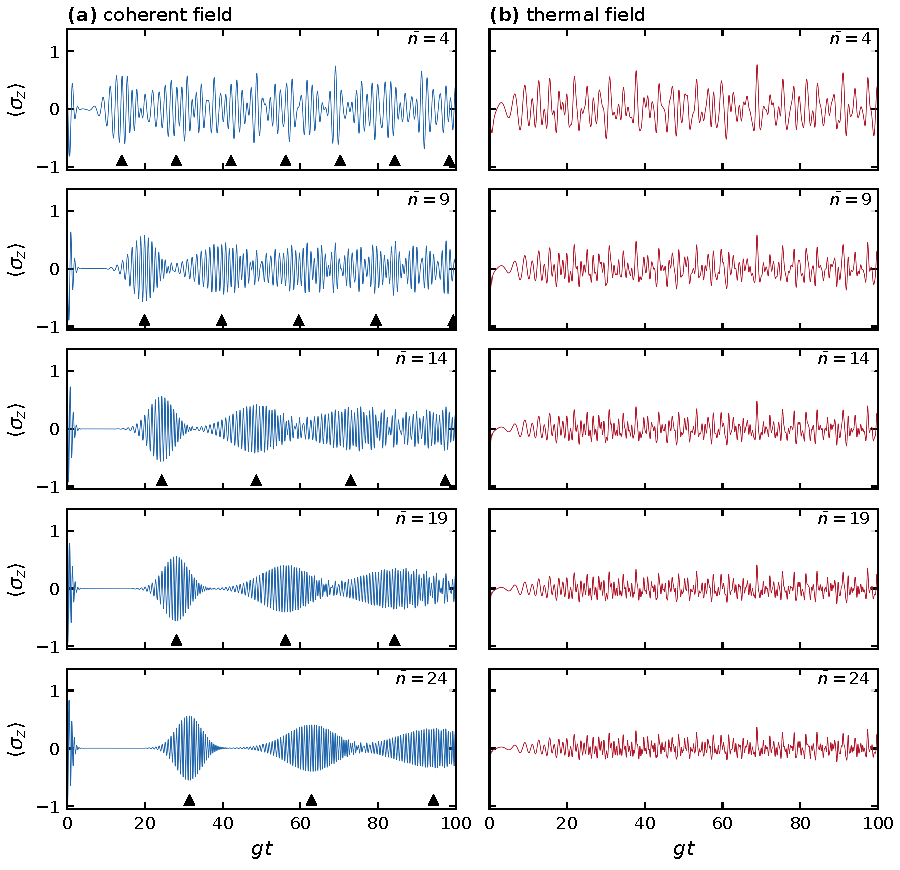
\includegraphics[width=6in]{jaynes_cummings_comparison.pdf}
    \caption{Atomic inversion $\sum_n p(n)\cos(2g\sqrt{n+1}\,t)$ for (a) coherent and (b) thermal fields with $\bar{n} = 4$, 9, 14, 19, and 24. Coherent fields show collapse--revival dynamics; the revivals, centered at multiples of $2\pi\sqrt{\bar{n}+1}/g$ (triangles), become more widely separated and better resolved as $\bar{n}$ increases. Thermal fields dephase within a Rabi period and then fluctuate irregularly, with spikes at multiples of $\pi/g$ where the components with $n + 1$ a perfect square rephase.}
    \label{fig:rabi_collapse_revival}
\end{figure*}

For a thermal field, with the Bose--Einstein photon statistics $p(n) = \bar{n}^n/(1+\bar{n})^{n+1}$, the distribution is much broader than the Poisson distribution ($\sigma_n \sim \bar{n}$ rather than $\sqrt{\bar{n}}$). The dephasing is correspondingly faster, and what follows is an irregular signal of overlapping partial revivals, with no well-defined revival sequence~\cite{knight1982}; the evolution nevertheless remains unitary, so this is a loss of visibility rather than a strictly irreversible process.\revtexonly{ Figure~\ref{fig:rabi_collapse_revival} shows the sum in Eq.~(\ref{eq:pe_cos_sum}) evaluated for both photon-number distributions.} This contrast between coherent and thermal fields is examined numerically in Sec.~\ref{sec:entropy_results}.

During the collapse the atom and field become strongly entangled. At half the revival time, $t_r/2 = \pi\sqrt{\bar{n}}/g$, the two branches of the atomic state reconverge onto a common state that is independent of the initial atomic state, so that the atom and field approximately disentangle, and the field is left in a nearly pure Schr\"{o}dinger cat state, a superposition of two components of opposite phase, each close to a coherent state~\cite{gea-banacloche1990, gea-banacloche1991, phoenix1991}. The connection between the Rabi collapse, transient entanglement, half-revival disentanglement, and cat-state formation is the subject of Sec.~\ref{sec:results}.


\subsection{Dressed-state spectroscopy}
\label{sec:dressed_spectroscopy}

\begin{figure}[tb]
    \centering
    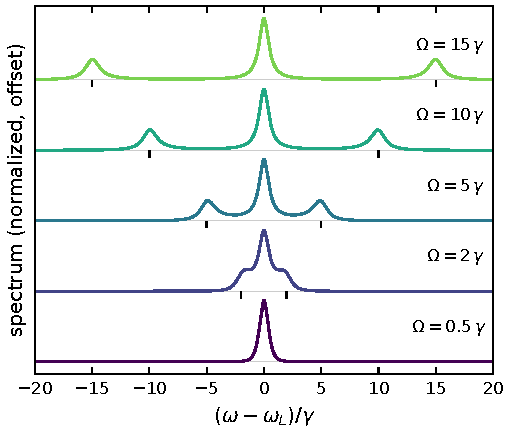
\includegraphics[width=\columnwidth]{mollow_triplet_driving_strength.pdf}
    \caption{Incoherent resonance-fluorescence spectra of a two-level atom of natural linewidth $\gamma$ driven resonantly at the frequency $\omega_L$, for Rabi frequencies $\Omega/\gamma = 0.5$, 2, 5, 10, and 15, each normalized to its peak and offset vertically. As the driving strength increases the single peak splits into the Mollow triplet: a central line and two sidebands at $\omega - \omega_L \approx \pm\Omega$ (ticks), with peak heights in the ratio $1{:}3{:}1$ for $\Omega \gg \gamma$.}
    \label{fig:mollow_triplet}
\end{figure}

The dressed-state picture also explains spectroscopic signatures of strong atom--field coupling. In resonance fluorescence of a strongly driven two-level atom, the emission spectrum exhibits a central peak at the drive frequency $\omega_L$ and sidebands at $\omega_L \pm \Omega$, where $\Omega$ is the Rabi frequency of the drive. This is the Mollow triplet~\cite{mollow1969}\revtexonly{ (Fig.~\ref{fig:mollow_triplet})}, which can be interpreted as transitions between dressed states separated by $\hbar\Omega$. In cavity QED, a strongly coupled atom--cavity system shows normal-mode splitting: the cavity transmission spectrum splits into two peaks at $\omega_c \pm g$ for one excitation, a direct observation of the single-excitation ($n = 0$) dressed-state splitting of $2g$~\cite{thompson1992}. As $n$ increases, the splitting grows as $\sqrt{n+1}$, though thermal fluctuations may blur individual $n$-dependent peaks in practice.


\subsection{Open quantum systems: The Lindblad master equation}
\label{sec:lindblad}

Real cavity QED systems are coupled to their environment. The dominant dissipation channels are cavity photon loss at rate $\kappa$ and atomic spontaneous emission into noncavity modes at rate $\gamma$. Within the Markov approximation, the density matrix evolves according to the Lindblad master equation~\cite{lindblad1976, wiseman2009}:
\begin{equation}
\frac{d\rho}{dt} = -\frac{i}{\hbar}[H_{\text{JC}}, \rho] + \kappa\, \mathcal{D}[a]\rho + \gamma\, \mathcal{D}[\sigma^-]\rho,
\label{eq:lindblad}
\end{equation}
where the Lindblad dissipator is
\begin{equation}
\mathcal{D}[L]\rho = L\rho L^\dagger - \frac{1}{2}\big(L^\dagger L \rho + \rho L^\dagger L\big).
\label{eq:dissipator}
\end{equation}
The strong-coupling regime, where quantum coherent effects dominate, requires $g \gg \kappa, \gamma$ so that the atom and field exchange energy many times before dissipation destroys coherence. In this regime, vacuum Rabi splitting is spectroscopically resolvable and collapse--revival dynamics can unfold before being damped.

The cat states generated during JC dynamics are especially sensitive to dissipation. The interference fringes of a superposition of two coherent states $|\alpha_1\rangle$ and $|\alpha_2\rangle$ decohere at the rate $\kappa|\alpha_1 - \alpha_2|^2/2$~\cite{zurek2003, haroche2006}; for the JC cat state, whose components sit at $\pm i\sqrt{\bar{n}}$ (Sec.~\ref{sec:wigner_results}), this is $2\kappa\bar{n}$, far exceeding the bare cavity decay rate $\kappa$. This fragility is quantified in Sec.~\ref{sec:decoherence}.


\subsection{Atom--field entanglement measures}
\label{sec:entropy_theory}

For a pure state $|\Psi\rangle$ of the atom--field system, the degree of entanglement is uniquely quantified by the von Neumann entropy of either reduced state~\cite{nielsen2000}:
\begin{equation}
S(\rho_{\text{atom}}) = -\mathrm{Tr}\big[\rho_{\text{atom}} \log_2 \rho_{\text{atom}}\big],
\label{eq:entropy}
\end{equation}
where $\rho_{\text{atom}} = \mathrm{Tr}_{\text{field}}[|\Psi\rangle\langle\Psi|]$. For a two-level atom, $S$ ranges from 0 (product state) to 1~bit (maximally entangled). The entropy is related to the purity of the reduced field state,
\begin{equation}
\mathcal{P} = \mathrm{Tr}\big[\rho_{\text{field}}^2\big],
\label{eq:purity}
\end{equation}
where $\rho_{\text{field}} = \mathrm{Tr}_{\text{atom}}[|\Psi\rangle\langle\Psi|]$; the purity equals unity for product states and decreases with increasing entanglement.

Equation~(\ref{eq:entropy}) is an entanglement measure only when the global atom--field state is pure. If the global state is mixed, as for a thermal initial field or whenever dissipation acts, $S(\rho_{\text{atom}})$ measures only the mixedness of the atom, which can arise from classical correlations with the field or from correlations with the environment as well as from atom--field entanglement, and it can saturate at 1~bit for a weakly entangled state. In those cases we use the logarithmic negativity~\cite{vidal2002, plenio2005}
\begin{equation}
E_{\mathcal{N}} = \log_2 \big\| \rho^{T_{\text{atom}}} \big\|_1,
\label{eq:logneg}
\end{equation}
where $T_{\text{atom}}$ denotes partial transposition with respect to the atom and $\|\cdot\|_1$ the trace norm. The logarithmic negativity is an entanglement monotone for mixed states; it vanishes for separable states and equals 1 for a maximally entangled atom--field pair.

In the JC model, the entanglement dynamics are directly correlated with the collapse and revival of Rabi oscillations~\cite{phoenix1988}. As the oscillations collapse, the atom becomes strongly entangled with the field ($S \to 1$~bit). At half the revival time, however, the system approximately refactorizes: $S$ passes through a minimum, the atom approaches a pure state, and the field is left in a nearly pure cat-like state~\cite{gea-banacloche1990, phoenix1991}. Around the full revival the branches rephase and the entanglement grows again. This entropy--inversion correspondence was first analyzed by Phoenix and Knight~\cite{phoenix1988, phoenix1991}, and we verify it computationally in Sec.~\ref{sec:results}.


%% ============================================================
%% SECTION 3: COMPUTATIONAL METHODS
%% ============================================================
\section{Computational Methods}
\label{sec:methods}

All simulations are performed using QuTiP (Quantum Toolbox in Python, version~5.2.3)~\cite{johansson2012, johansson2013}, an open-source framework for simulating open and closed quantum systems. The cavity field is represented in a truncated Fock basis $\{|0\rangle, |1\rangle, \ldots, |N_{\text{cav}}-1\rangle\}$, and the joint atom--field Hilbert space has dimension $2N_{\text{cav}}$.

\textit{Fock-space truncation.} The truncation is chosen per initial state. For the coherent and Fock states with $\bar{n} = 10$ we use $N_{\text{cav}} = 35$--$50$: the Poisson weight beyond $n = 35$ is below $10^{-9}$, and every quantity reported at $t_r/2$ (entropy, purity, $\delta$) agrees to better than $10^{-4}$ for $N_{\text{cav}} = 35$, 50, and 70. Thermal and squeezed-vacuum fields have much heavier photon-number tails (geometric, and $\propto \tanh^{2m}r/\sqrt{m}$ for $n = 2m$, respectively): at $N_{\text{cav}} = 50$ the truncated states would have $\langle\hat{n}\rangle = 9.57$ (thermal) and $8.23$ (squeezed vacuum) instead of 10. We therefore use $N_{\text{cav}} = 150$ for the thermal field and $N_{\text{cav}} = 300$ for the squeezed vacuum, which reproduce $\langle\hat{n}\rangle = 10$ to four digits and leave a truncated weight below $10^{-6}$ (for the squeezed vacuum the weight beyond $n = 150$ is still $1.6\times10^{-4}$); the squeezed vacuum is built from its exact Fock amplitudes. For the $\bar{n}$ scan we use $N_{\text{cav}} = 3\bar{n} + 20$. Trace normalization alone is not used as a convergence criterion.

\textit{Time evolution.} All propagation uses QuTiP's \texttt{mesolve} with its default adaptive-step Adams--Moulton multistep integrator (\texttt{method='adams'}, absolute and relative tolerances $10^{-8}$ and $10^{-6}$). Pure initial states without dissipation are propagated as state vectors; for the thermal initial field and for all dissipative runs [Eq.~(\ref{eq:lindblad})] the full density matrix is propagated.

\textit{Wigner functions.} At each snapshot time, we obtain the reduced field state $\rho_{\text{field}}(t) = \mathrm{Tr}_{\text{atom}}[\rho(t)]$ via partial trace, then compute $W(x,p)$ on a $281 \times 281$ grid over $[-7, 7]^2$ (spacing 0.05, i.e., 14 points per interference fringe of spacing $\pi/\sqrt{2\bar{n}} \approx 0.70$) using QuTiP's \texttt{wigner} function~\cite{johansson2012} in the convention $a = (x + ip)/\sqrt{2}$, for which $\int W\,dx\,dp = 1$ (verified to $3\times10^{-4}$ on the grid, the residual being the tail outside the window). The Wigner negativity $\delta$ of Eq.~(\ref{eq:negativity}) is evaluated on the same grid; halving or doubling the spacing changes it by less than $2\times10^{-3}$. For the map over the $(\bar{n}, \kappa/g)$ plane in Sec.~\ref{sec:decoherence} the window is enlarged to $\pm(\sqrt{2\bar{n}} + 4.5)$ at a comparable spacing. All Wigner function maps share one color scale, $|W| \leq 1/\pi$, the bound for any state in this convention.

\textit{Entanglement and cat-state measures.} The von Neumann entropy $S(\rho_{\text{atom}})$ is computed at each time step from the eigenvalues of the $2 \times 2$ reduced atomic density matrix, the field purity $\mathcal{P}(t) = \mathrm{Tr}[\rho_{\text{field}}^2]$ directly, and the logarithmic negativity of Eq.~(\ref{eq:logneg}) from the trace norm of the partially transposed global state; for a pure global state with Schmidt probabilities $\lambda_{1,2}$ it reduces to $E_{\mathcal{N}} = \log_2(1 + 2\sqrt{\lambda_1\lambda_2})$, a monotonic function of $S$. The cat-state fidelity is $F_{\text{cat}} = \max\,\langle \text{cat}|\rho_{\text{field}}|\text{cat}\rangle$ over normalized states $|\text{cat}\rangle \propto |\beta\rangle + e^{i\chi}|{-\beta}\rangle$, with $\beta$ scanned in a neighborhood of $i\sqrt{\bar{n}}$ and $\chi \in [0, 2\pi)$.

\textit{Parameters.} We work on resonance and in the interaction picture, i.e., in the frame rotating at $\omega_c = \omega_a$, where the Hamiltonian is $\hbar g(a^\dagger\sigma^- + a\,\sigma^+)$; all field states and Wigner functions are given in this frame. We use dimensionless units with $g = 1$. The characteristic timescales are the collapse time $t_c \equiv 1/g$ and the revival time $t_r = 2\pi\sqrt{\bar{n}}/g$. Table~\ref{tab:params} summarizes the simulation parameters.

\begin{table}[tb]
\caption{Simulation parameters. Rates are in units of $g$; atomic decay is neglected ($\gamma = 0$) in all runs.}
\label{tab:params}
\begin{ruledtabular}
\begin{tabular}{lccc}
Simulation & $\bar{n}$ & $N_{\text{cav}}$ & $\kappa/g$ \\
\hline
Wigner evolution & 10 & 35 & 0 \\
Entanglement (coherent, Fock) & 10 & 50 & 0 \\
Entanglement (thermal) & 10 & 150 & 0 \\
Entanglement (squeezed vacuum) & 10 & 300 & 0 \\
$\bar{n}$ scaling & 1--36 & $3\bar{n}+20$ & 0 \\
Dissipative dynamics & 10 & 35--50 & 0--0.20 \\
Cat-survival map & 1--25 & $3\bar{n}+20$ & 0.001--0.20 \\
\end{tabular}
\end{ruledtabular}
\end{table}


%% ============================================================
%% SECTION 4: RESULTS AND DISCUSSION
%% ============================================================
\section{Results and Discussion}
\label{sec:results}

\subsection{Wigner function evolution and cat-state formation}
\label{sec:wigner_results}

\begin{figure*}[t]
    \centering
    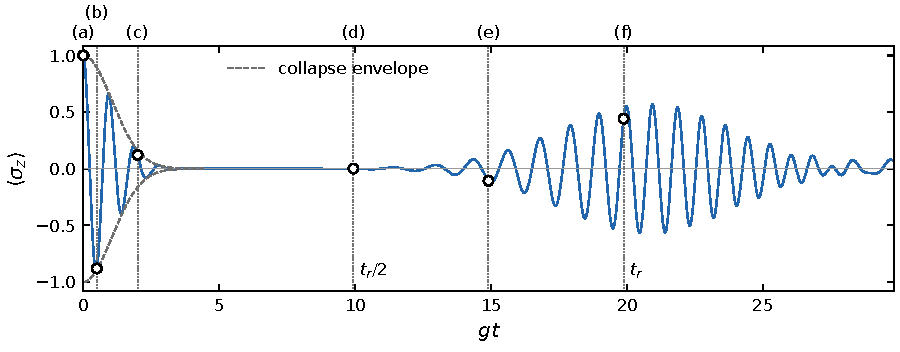
\includegraphics[width=6in]{fig_inversion_snapshots.pdf}
    \caption{Atomic inversion $\langle\sigma_z\rangle$ for an initially excited two-level atom interacting with a coherent field ($\bar{n} = 10$) in the resonant Jaynes--Cummings model. Circles labeled (a)--(f) mark the times $gt = 0$, 0.5, 2, $gt_r/2$, $0.75\,gt_r$, and $gt_r$ [$t_r = 2\pi\sqrt{\bar{n}}/g \approx 19.9/g$] at which the Wigner function is shown in the corresponding panels of Fig.~\ref{fig:wigner_evolution}. The dashed curves are the collapse envelope $\pm\exp[-g^2t^2\bar{n}/2(\bar{n}+1)]$ of Sec.~\ref{sec:collapse_revival}.}
    \label{fig:inversion_snapshots}
\end{figure*}

We first consider unitary JC dynamics with the atom initially excited and the field in a coherent state $|\alpha\rangle$ with $\alpha = \sqrt{10}$, i.e., $\bar{n} = 10$. Figure~\ref{fig:inversion_snapshots} shows the atomic inversion $\langle\sigma_z\rangle$ with its collapse--revival structure: rapid Rabi oscillations that dephase within a few $1/g$ under the envelope of Sec.~\ref{sec:collapse_revival}; a quiescent interval; and a revival around $t_r \approx 19.9/g$, whose envelope peaks near $20.9/g$.

\begin{figure*}[t]
    \centering
    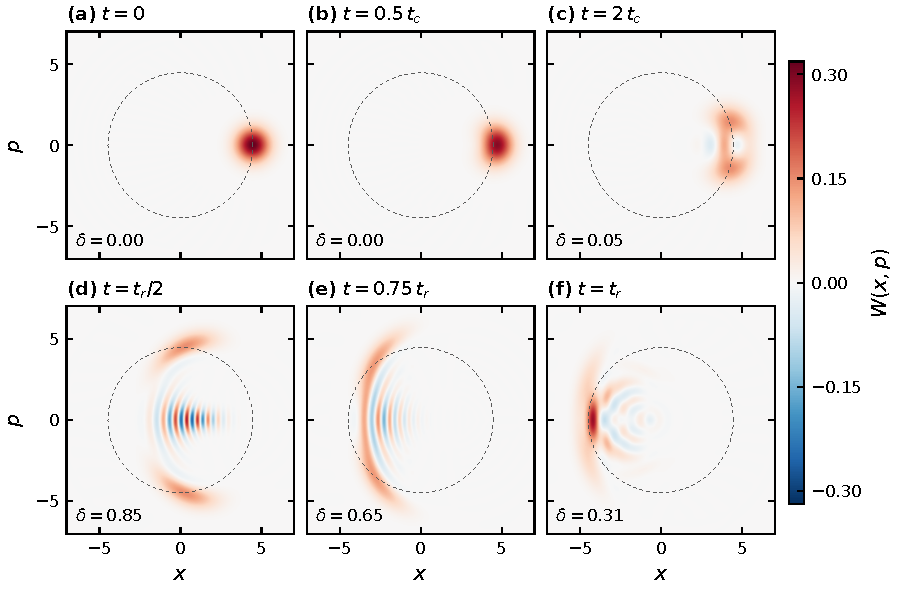
\includegraphics[width=6in]{fig_wigner_evolution.pdf}
    \caption{Wigner function $W(x,p)$ of the reduced cavity field during Jaynes--Cummings evolution ($\bar{n} = 10$, $\Delta = 0$), on a common color scale; the dashed circle is $x^2 + p^2 = 2\bar{n}$ and $\delta$ is the Wigner negativity. (a) $t = 0$, the initial coherent state. (b) $t = 0.5\,t_c$, with $t_c = 1/g$. (c) $t = 2\,t_c$: the field has split into two components moving in opposite directions along the circle, and the Rabi oscillations have largely collapsed. (d) $t = t_r/2$: the components sit at $p \approx \pm\sqrt{2\bar{n}}$ and are joined by interference fringes, a Schr\"{o}dinger cat state formed while the atom and field are approximately disentangled (Sec.~\ref{sec:entropy_results}). (e) $t = 0.75\,t_r$. (f) $t = t_r$: the components meet again and the field partially relocalizes.}
    \label{fig:wigner_evolution}
\end{figure*}

Figure~\ref{fig:wigner_evolution} shows the Wigner function of the reduced cavity field at six characteristic times. At $t = 0$, the Wigner function is a Gaussian displaced to $x \approx 4.5$, consistent with the initial coherent state. As the system evolves through the collapse, the distribution splits into two components that move in opposite directions along the circle $x^2 + p^2 = 2\bar{n}$, each at the angular velocity $g/(2\sqrt{\bar{n}})$~\cite{gea-banacloche1991}; the Rabi oscillations have collapsed once the two no longer overlap. At the midpoint of the collapse--revival cycle ($t = t_r/2$), the Wigner function develops two well-separated lobes connected by interference fringes with alternating positive and negative values, the signature of a Schr\"{o}dinger cat state, $|\Psi_{\text{cat}}\rangle \propto |\beta\rangle + e^{i\chi}|{-\beta}\rangle$ with $\beta \approx i\sqrt{\bar{n}}$: the two components sit on the $p$ axis, rotated by $\pm\pi/2$ from the initial coherent amplitude.

\begin{figure*}[t]
    \centering
    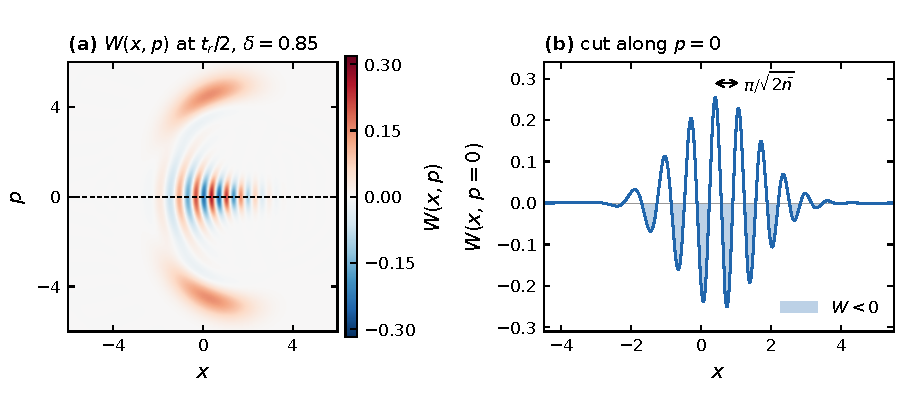
\includegraphics[width=6in]{fig_cat_state_detail.pdf}
    \caption{The Schr\"{o}dinger cat state formed at $t = t_r/2$ for $\bar{n} = 10$. (a) Wigner function, showing the two lobes and the interference fringes between them; the dashed line marks the cut used in (b). (b) $W(x, p = 0)$, with negative regions shaded, reaching $W \approx -0.25$; the arrow indicates the fringe spacing $\pi/\sqrt{2\bar{n}} \approx 0.70$. The Wigner negativity is $\delta = 0.85$ and the fidelity with the best-fitting two-component cat state is 0.78.}
    \label{fig:cat_detail}
\end{figure*}

Figure~\ref{fig:cat_detail} provides a detailed view of this cat state. The cut $W(x, 0)$ reaches $W \approx -0.25$, and the Wigner negativity of the state is $\delta = 0.85$ ($\delta = 0$ at $t = 0$). This exceeds the $\delta = 0.63$ of an ideal superposition of two coherent states of the same amplitude ($\delta \to 2/\pi \approx 0.64$ for well-separated components), because the two components produced by the JC dynamics are not coherent states: each is sheared into a squeezed, crescent-shaped state~\cite{gea-banacloche1991}. For the same reason the best-fitting two-component cat state has a fidelity of only $F_{\text{cat}} = 0.78$ with the reduced field state, although the purity of that state is $\mathcal{P} = 0.96$; the fidelity does not improve with the field size (it is 0.79 for $\bar{n} = 40$ and for $\bar{n} = 160$). The field is thus in a nearly pure cat-like state rather than in one branch of an entangled atom--field pair (Sec.~\ref{sec:entropy_results}). The relative phase of the fit is $\chi \approx 1.2\pi$ and the photon-number parity is $\langle(-1)^{\hat{n}}\rangle = -0.64$, so for $\bar{n} = 10$ the state is closer to an odd than to an even cat state. The sign is not universal: the parity at $t_r/2$ alternates with $\bar{n}$, $-0.64$ for even and $+0.64$ for odd integer $\bar{n}$, which is why the relative phase must be fitted rather than assumed. The fidelity with the even cat state $|\alpha\rangle + |{-\alpha}\rangle$ on the real axis is essentially zero. The interference fringes have the spacing $\pi/\sqrt{2\bar{n}} \approx 0.70$ (0.68 in the simulation), set by the separation of the two components. They are the phase-space signature of quantum interference between mesoscopically distinct field states and a direct signature of nonclassicality.

As the system approaches the revival time, the two lobes merge and the Wigner function partially relocalizes, though with residual nonclassical features ($\delta = 0.31$ at $t = t_r$). The revival is not exact: higher-order terms in the expansion of $\sqrt{n+1}$ about $\bar{n}$ prevent perfect rephasing.


\subsection{Atom--field entanglement dynamics}
\label{sec:entropy_results}

We now quantify atom--field entanglement, comparing four initial field states with the same mean photon number $\bar{n} = 10$: coherent, thermal, squeezed vacuum, and Fock. For the three pure initial fields the global state remains pure and $S(\rho_{\text{atom}})$ is the entanglement entropy. We report $S$ and the logarithmic negativity $E_{\mathcal{N}}$ of Eq.~(\ref{eq:logneg}) in all four cases; for the thermal field only $E_{\mathcal{N}}$ measures entanglement.

\begin{figure*}[t]
    \centering
    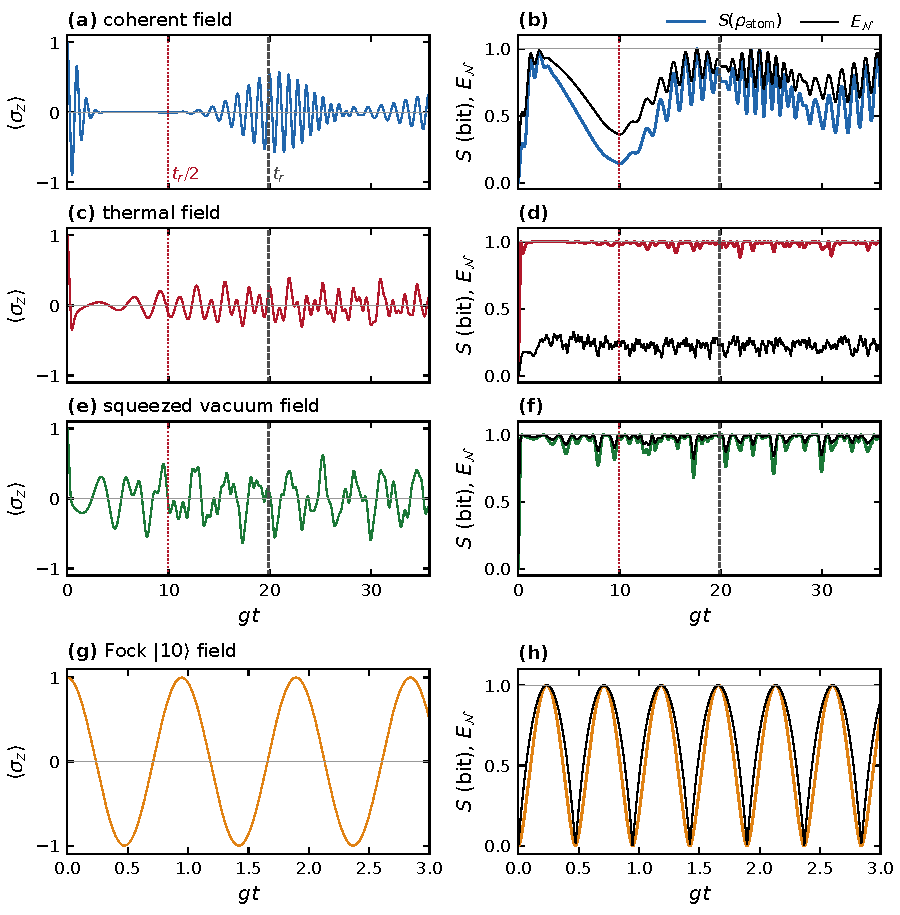
\includegraphics[width=6in]{fig_entanglement_comparison.pdf}
    \caption{Jaynes--Cummings dynamics for four initial field states with $\bar{n} = 10$. Left column: atomic inversion $\langle\sigma_z\rangle$. Right column: reduced atomic entropy $S(\rho_{\text{atom}})$ (colored) and logarithmic negativity $E_{\mathcal{N}}$ (thin black). (a), (b) Coherent field: $S$ rises to about 1~bit during the collapse and falls to its minimum near $t_r/2$ (dotted vertical line), where the atom and field approximately disentangle; the dashed vertical line marks $t_r$. (c), (d) Thermal field: $S$ stays close to 1~bit but $E_{\mathcal{N}} \approx 0.2$, because the global state is mixed. (e), (f) Squeezed vacuum: only partial dips. (g), (h) Fock state $|10\rangle$, on a shorter time axis: the inversion oscillates with period $\pi/(g\sqrt{11})$ and $S$ with half that period. For the three pure initial fields $E_{\mathcal{N}}$ and $S$ are functions of the same Schmidt probabilities.}
    \label{fig:entanglement_comparison}
\end{figure*}

Figure~\ref{fig:entanglement_comparison} shows the inversion, the reduced atomic entropy, and the logarithmic negativity for all four cases. The principal observations are as follows.

\textit{Coherent state.} The entropy rises from $S = 0$ to about 1~bit within $t \approx 2/g$, as the Rabi oscillations collapse. It then decreases steadily and reaches a minimum $S \approx 0.14$~bit ($E_{\mathcal{N}} = 0.36$) close to $t_r/2 \approx 9.9/g$ (at $gt \approx 10.0$), in the middle of the quiescent interval. This is the half-revival disentanglement predicted by Gea-Banacloche~\cite{gea-banacloche1990}: the atom returns close to a pure state while the field is in the cat state of Fig.~\ref{fig:cat_detail}. Toward the revival the entanglement grows again; around $t_r$ the entropy oscillates between about 0.5 and 1~bit at the Rabi frequency ($S \approx 0.79$~bit at $t_r$).

\textit{Thermal state.} The reduced atomic entropy rises to $S = 1$~bit within $t \sim 1/g$ and stays close to the maximum thereafter (0.985~bit on average, with brief dips to 0.88~bit), with no dip at $t_r/2$. This does not indicate maximal entanglement: the global state is mixed, and the logarithmic negativity remains small, $E_{\mathcal{N}} \approx 0.23$ on average (maximum 0.33). Most of the reduced atomic entropy therefore reflects classical correlations with the mixed initial field rather than entanglement. The broad Bose--Einstein photon distribution ($\sigma_n \sim \bar{n}$) spreads the Rabi frequencies, dephases the oscillations within a Rabi period, and leaves an irregular signal in which no individual revival is resolved~\cite{knight1982}.

\textit{Squeezed vacuum.} The dynamics are intermediate: a rapid rise to about 1~bit followed by quasiperiodic partial dips (to $S \approx 0.7$--$0.8$~bit), but no clear half-revival disentanglement. The super-Poissonian photon statistics of the squeezed vacuum (only even $n$ populated, variance $2\bar{n}(\bar{n}+1)$) spread the Rabi frequencies over a much wider range than the Poisson distribution does.

\textit{Fock state.} With a definite photon number there is a single Rabi frequency, $\Omega_{10} = 2g\sqrt{11}$ [Eq.~(\ref{eq:gen_rabi}) with $\Delta = 0$]. The inversion oscillates with period $\pi/(g\sqrt{11}) \approx 0.95/g$, and the entropy, $S = h(P_e)$ with the binary entropy $h(x) = -x\log_2 x - (1-x)\log_2(1-x)$, oscillates between 0 and 1~bit with half that period, $\pi/(2g\sqrt{11}) \approx 0.47/g$ [Figs.~\ref{fig:entanglement_comparison}(g) and \ref{fig:entanglement_comparison}(h)]. No collapse or revival occurs because there is no dephasing.

\begin{figure*}[t]
    \centering
    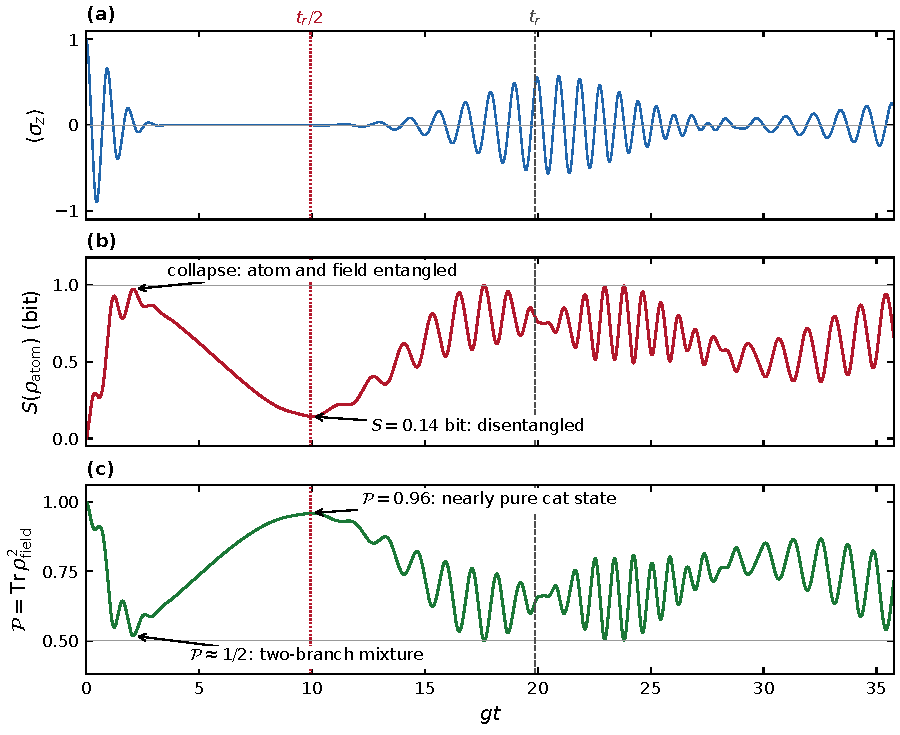
\includegraphics[width=6in]{fig_coherent_entropy_purity.pdf}
    \caption{Coherent-state dynamics in detail ($\bar{n} = 10$). (a) Atomic inversion. (b) Reduced atomic entropy $S(\rho_{\text{atom}})$, peaking near 1~bit during the collapse and reaching its minimum (0.14~bit) near $t_r/2$, where the atom and field approximately disentangle and the field is in the cat state of Fig.~\ref{fig:cat_detail}. (c) Field purity $\mathcal{P} = \mathrm{Tr}[\rho_{\text{field}}^2]$, dropping to about $1/2$ during the collapse (a two-branch mixture, the field being entangled with the atom) and rising to 0.96 at $t_r/2$ (nearly pure cat-like state). Dotted and dashed lines mark $t_r/2$ and $t_r$.}
    \label{fig:coherent_detail}
\end{figure*}

Figure~\ref{fig:coherent_detail} shows the coherent-state case in greater detail, with the inversion, the entropy, and the field purity $\mathcal{P}(t)$ together. During the collapse the field purity drops to $\mathcal{P} \approx 1/2$: the reduced field is then an incoherent mixture of two nearly orthogonal branches, each correlated with a different atomic state (a coherent superposition of the two branches would have $\mathcal{P} = 1$). As the atomic branches reconverge, the purity climbs to $\mathcal{P} = 0.96$ at $t_r/2$, where the field is in the nearly pure cat-like state, and falls again toward the revival ($\mathcal{P} = 0.64$ at $t_r$). The three observables give a consistent picture: entanglement during the collapse turns the reduced field into a two-branch mixture, and disentanglement at $t_r/2$ restores the coherence of the field in the form of a cat state.

\begin{figure*}[t]
    \centering
    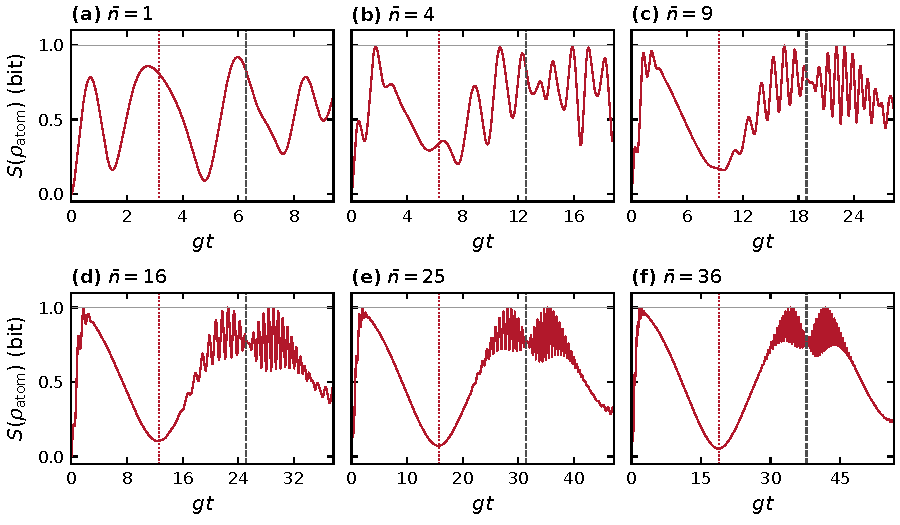
\includegraphics[width=6in]{fig_entropy_nbar_scaling.pdf}
    \caption{Reduced atomic entropy $S(\rho_{\text{atom}})$ for coherent fields with (a)--(f) $\bar{n} = 1$, 4, 9, 16, 25, and 36. As $\bar{n}$ increases, the collapse time remains of order $1/g$ while the half-revival time $\pi\sqrt{\bar{n}}/g$ (dotted) and the revival time $t_r = 2\pi\sqrt{\bar{n}}/g$ (dashed) grow as $\sqrt{\bar{n}}$. The entropy minimum near $t_r/2$ (approximate atom--field disentanglement) deepens with $\bar{n}$ and is well resolved for $\bar{n} \gtrsim 9$.}
    \label{fig:entropy_nbar}
\end{figure*}

Figure~\ref{fig:entropy_nbar} shows how these dynamics depend on $\bar{n}$. For $\bar{n} = 1$ the entropy oscillates quasiperiodically without a clear collapse. As $\bar{n}$ increases, the collapse still occurs at $t \sim 1/g$, but the half-revival minimum near $\pi\sqrt{\bar{n}}/g$ shifts to later times and deepens ($S_{\min} \approx 0.16$, 0.10, 0.07, and 0.05~bit for $\bar{n} = 9$, 16, 25, and 36), and the entangled plateau around the revival broadens. For $\bar{n} \gtrsim 9$ the disentanglement and the subsequent reentanglement are well resolved, consistent with the large-$\bar{n}$ analysis of Gea-Banacloche~\cite{gea-banacloche1991}.


\subsection{Decoherence of nonclassical features}
\label{sec:decoherence}

We now include cavity photon loss ($\kappa > 0$) via Eq.~(\ref{eq:lindblad}) and study its effect on the Wigner function and entanglement.

\begin{figure*}[t]
    \centering
    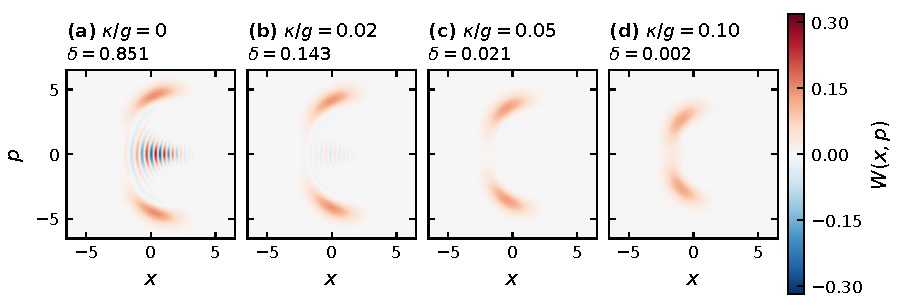
\includegraphics[width=6in]{fig_wigner_decoherence.pdf}
    \caption{Decoherence of the Schr\"{o}dinger cat state ($\bar{n} = 10$): Wigner function at $t = t_r/2$ for the cavity decay rates (a) $\kappa/g = 0$, (b) 0.02, (c) 0.05, and (d) 0.10, on the color scale of Fig.~\ref{fig:wigner_evolution}. The interference fringes disappear while the two lobes survive; $\delta$ is the Wigner negativity (Table~\ref{tab:decoherence}).}
    \label{fig:wigner_decoherence}
\end{figure*}

Figure~\ref{fig:wigner_decoherence} shows the Wigner function at $t = t_r/2$ for $\kappa/g = 0$, 0.02, 0.05, and 0.10. The interference fringes are progressively destroyed: at $\kappa/g = 0.02$ the Wigner negativity drops from $\delta = 0.85$ to $\delta = 0.14$, and at $\kappa/g = 0.10$ it is effectively zero ($\delta = 0.002$). Table~\ref{tab:decoherence} summarizes these results; the values agree to three digits for $N_{\text{cav}} = 35$ and 50.

\begin{table}[tb]
\caption{Wigner negativity $\delta$, its ratio to the lossless value, and field purity $\mathcal{P}$ at $t = t_r/2$ for several cavity decay rates, with $\bar{n} = 10$.}
\label{tab:decoherence}
\begin{ruledtabular}
\begin{tabular}{cccc}
$\kappa/g$ & $\delta$ & $\delta(\kappa)/\delta(0)$ & $\mathcal{P}$ \\
\hline
0.00 & 0.851 & 1.00 & 0.960 \\
0.02 & 0.143 & 0.17 & 0.460 \\
0.05 & 0.021 & 0.03 & 0.418 \\
0.10 & 0.002 & 0.00 & 0.386 \\
\end{tabular}
\end{ruledtabular}
\end{table}

This sensitivity can be estimated simply; the decoherence of the JC cat state under cavity loss was analyzed in Refs.~\cite{gea-banacloche1993, meunier2006}. The fringe decoherence rate is $\kappa|\alpha_1 - \alpha_2|^2/2$ (Sec.~\ref{sec:lindblad}), and the two components separate gradually, $|\alpha_1 - \alpha_2| = 2\sqrt{\bar{n}}\,\sin[gt/(2\sqrt{\bar{n}})]$, so the rate grows from zero to $2\kappa\bar{n}$ at $t_r/2$ and its time integral is $\pi\kappa\bar{n}^{3/2}/g$. The fringe visibility, and with it the Wigner negativity, is therefore reduced approximately by
\begin{equation}
\frac{\delta(\kappa)}{\delta(0)} \approx \exp\!\left(-\frac{\pi\kappa\,\bar{n}^{3/2}}{g}\right),
\label{eq:visibility}
\end{equation}
where $\delta(\kappa)$ is the Wigner negativity at $t_r/2$ for the decay rate $\kappa$. For $\bar{n} = 10$ and $\kappa/g = 0.02$ this gives 0.137, close to the simulated ratio 0.168. The two lobes decay only at the rate $\kappa$ and persist. Using the final rate $2\kappa\bar{n}$ for the whole interval would double the exponent and predict a 98\% loss instead of the 83\% observed. At larger $\kappa$ the simulated Wigner negativity lies above Eq.~(\ref{eq:visibility}), since the amplitude decay reduces the separation and part of $\delta$ resides in the deformed lobes rather than in the fringes.

\begin{figure*}[t]
    \centering
    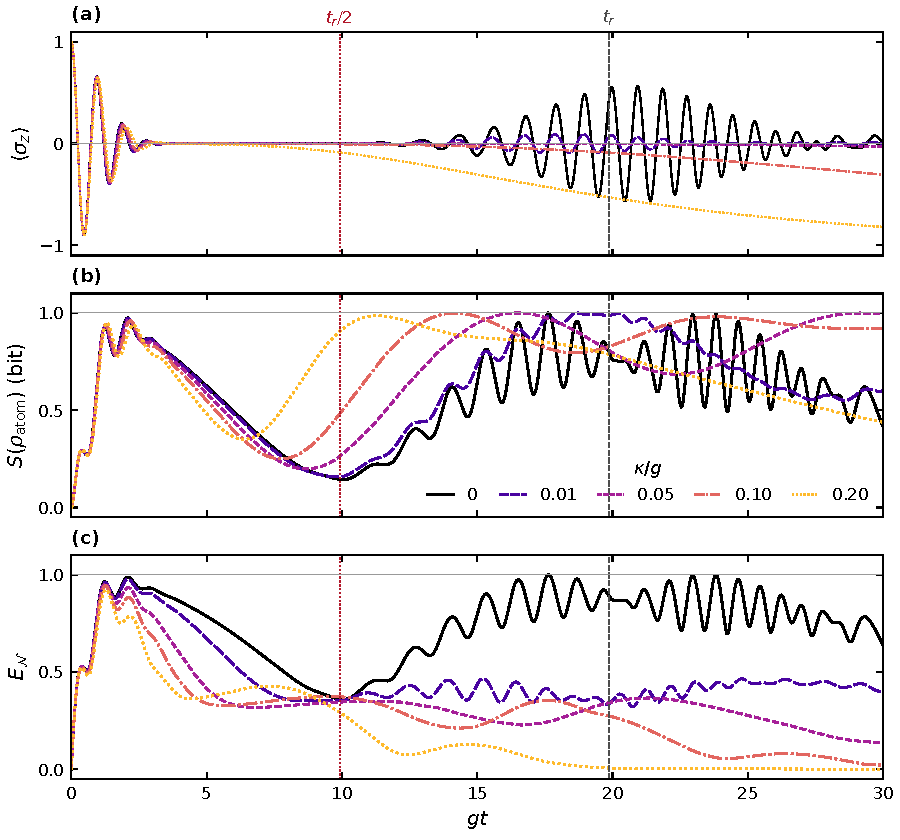
\includegraphics[width=6in]{fig_dissipative_entanglement.pdf}
    \caption{Effect of cavity decay on the JC dynamics ($\bar{n} = 10$) for $\kappa/g = 0$, 0.01, 0.05, 0.10, and 0.20 (dark to light; line styles as in the legend). (a) Atomic inversion. (b) Reduced atomic entropy, which for $\kappa > 0$ is no longer an entanglement measure. (c) Logarithmic negativity $E_{\mathcal{N}}$, an entanglement monotone for the mixed states produced by dissipation. Increasing $\kappa$ damps the revival, drives the atom toward its ground state, and suppresses the late-time logarithmic negativity even where the reduced entropy stays near 1~bit. Dotted and dashed vertical lines mark $t_r/2$ and $t_r$.}
    \label{fig:dissipative_entropy}
\end{figure*}

Figure~\ref{fig:dissipative_entropy} shows the inversion, the reduced atomic entropy, and the logarithmic negativity under dissipation. Three effects are visible. (i) The Rabi revival is damped and the inversion relaxes toward $\langle\sigma_z\rangle = -1$ as photons leak out; for $\kappa/g = 0.20$, $\langle\sigma_z\rangle = -0.82$ at $gt = 30$. (ii) The reduced atomic entropy no longer measures entanglement: at $gt = 30$ it is still 0.99 and 0.92~bit for $\kappa/g = 0.05$ and 0.10, where the logarithmic negativity has fallen to $E_{\mathcal{N}} = 0.14$ and 0.02; for $\kappa/g = 0.20$ both decay ($S = 0.44$~bit, $E_{\mathcal{N}} = 0.00$) as the atom relaxes to its ground state. (iii) The atom--field entanglement at $t_r/2$ is comparatively robust: $E_{\mathcal{N}}(t_r/2) = 0.35$--$0.37$ for all $\kappa/g \leq 0.10$, close to the unitary value 0.36, even though the entropy minimum is progressively filled in [$S(t_r/2) = 0.14$, 0.16, 0.26, and 0.48~bit for $\kappa/g = 0$, 0.01, 0.05, and 0.10] and the interference fringes are already gone at $\kappa/g = 0.05$ (Table~\ref{tab:decoherence}). Cavity loss thus destroys the internal coherence of the field cat state long before it changes the small residual entanglement between atom and field.

By the operational criterion $\delta > 0.05$ at $t_r/2$, cat-state formation with $\bar{n} = 10$ requires $\kappa/g \lesssim 0.03$, i.e., $g/\kappa \gtrsim 30$; the threshold depends on $\bar{n}$, on the observation time, and on the chosen figure of merit. For $\bar{n} \geq 10$ the threshold falls as $\bar{n}^{-1.4}$, approaching the $\bar{n}^{-3/2}$ scaling of Eq.~(\ref{eq:visibility}); a map of $\delta$ and $F_{\text{cat}}$ over the $(\bar{n}, \kappa/g)$ plane is included with the code~\cite{nguyen2026code}. This condition is met in microwave cavity QED~\cite{haroche2006} and circuit QED~\cite{blais2021}, but remains an engineering challenge in optical cavities.


%% ============================================================
%% SECTION 5: CLASSICAL VS QUANTUM CRITERIA
%% ============================================================
\section{Criteria for nonclassical light}
\label{sec:criteria}

The computational results above illustrate the distinction between classical and quantum light in a dynamical setting. Here we summarize the formal criteria and their relevance to quantum technologies.

The Glauber--Sudarshan $P$ function~\cite{glauber1963, sudarshan1963} provides the defining criterion. If the density operator of a state can be written as $\rho = \int P(\alpha) |\alpha\rangle\langle\alpha|\,d^2\alpha$ with a nonnegative, well-behaved $P(\alpha)$, the state is classical (a mixture of coherent states). States for which $P(\alpha)$ is more singular than a delta function or takes negative values, including Fock states and squeezed states, are nonclassical. Negativity of the Wigner function is sufficient but not necessary; the Husimi $Q$ function is nonnegative for every state and cannot serve as a witness.

Photon statistics provide experimentally accessible tests. Sub-Poissonian statistics [second-order coherence $g^{(2)}(0) < 1$] and photon antibunching [$g^{(2)}(\tau) > g^{(2)}(0)$] cannot occur with classical fields. The observation of photon antibunching in resonance fluorescence~\cite{kimble1977} is widely regarded as the first clear demonstration of nonclassical light. Conversely, photon bunching [$g^{(2)}(0) = 2$] is expected for thermal light and does not imply nonclassicality.

Squeezing below the vacuum level is another sufficient criterion for nonclassicality: no classical state has less noise in any quadrature than the vacuum. During the third observing run, the injection of squeezed vacuum into the Advanced LIGO detectors reduced the quantum shot noise by up to about 3~dB at frequencies above about 50~Hz, which was estimated to raise the detection rate for binary-neutron-star mergers by 40--50\%~\cite{tse2019}.

Nonclassical light is a resource for quantum technologies: squeezed states improve interferometric sensitivity beyond the standard quantum limit; entangled photon pairs enable quantum key distribution~\cite{ekert1991}; and NOON states of $N$ photons can achieve a Heisenberg-limited phase sensitivity scaling as $1/N$ rather than the shot-noise scaling $1/\sqrt{N}$.


%% ============================================================
%% SECTION 6: CONNECTION TO EXPERIMENT
%% ============================================================
\section{Connection to Experiment}
\label{sec:experiment}

The revivals were predicted by Eberly et al.\ in 1980~\cite{eberly1980} and first observed in 1987~\cite{rempe1987}. The observation required isolating a single two-level atom in a single-mode cavity in the strong-coupling regime ($g \gg \kappa, \gamma$).

\textit{Microwave cavity QED.} The first observation of quantum revivals was achieved by Rempe, Walther, and Klein~\cite{rempe1987} using a one-atom maser: Rydberg atoms, with transition frequencies in the microwave range, passed one at a time through a high-quality superconducting niobium cavity containing a weak thermal and maser field. The atoms entered in the upper state, and their final state was measured by field ionization as a function of the interaction time. The measured $P_e(t)$ exhibited the predicted collapse of the Rabi oscillations followed by a revival, in agreement with JC theory. Rabi oscillations in a small coherent field, with the discrete frequencies $\Omega_0\sqrt{n+1}$ individually resolved, were later observed by Brune et al.~\cite{brune1996rabi}. On a related platform, circular Rydberg atoms crossing an open superconducting Fabry--P\'{e}rot cavity, Haroche, Raimond, and collaborators~\cite{haroche2006} generated and detected Schr\"{o}dinger cat states by dispersive atom--field coupling~\cite{brune1996}, observed the splitting of a resonant coherent field into two components~\cite{auffeves2003}, recorded quantum jumps of the photon number~\cite{gleyzes2007}, and counted photons without destroying them~\cite{guerlin2007}. In these experiments the vacuum Rabi frequency is $\Omega_0/2\pi \approx 50$~kHz, i.e., $g/2\pi \approx 25$~kHz in the convention of Eq.~(\ref{eq:2x2}). The cavity damping time was below 1~ms in the earlier experiments (0.85~ms in Ref.~\cite{auffeves2003}, giving $g/\kappa \approx 130$) and reached 0.13~s, i.e., $\kappa/2\pi \approx 1.2$~Hz and $g/\kappa \approx 2\times10^4$, in 2007~\cite{gleyzes2007}.

\textit{Trapped ions.} The JC Hamiltonian also describes a trapped ion whose internal levels are coupled to its quantized motion by laser light tuned to a motional sideband. Meekhof et al.~\cite{meekhof1996} observed the collapse and a revival of Rabi oscillations in a single trapped $^9\text{Be}^+$ ion, using two hyperfine ground states coupled to the motion by stimulated Raman transitions. The vibrational mode of the ion played the role of the cavity field: they prepared it in a coherent state of motion with $\bar{n} \approx 3$ and drove the first blue sideband (the anti-JC coupling, equivalent to the JC coupling with the internal states interchanged). This experiment showed that the same dynamics arise for any two-level system coupled to a quantized bosonic mode.

\textit{Optical cavities.} In the optical domain, Thompson, Rempe, and Kimble~\cite{thompson1992} observed the vacuum Rabi splitting in the transmission spectrum of a high-finesse Fabry--P\'{e}rot cavity traversed by a cesium atomic beam with, on average, one atom in the mode, confirming the dressed-state structure of the single-excitation manifold. Time-domain collapse--revival experiments in optical cavities are more challenging because of the shorter cavity lifetimes.

\textit{Circuit QED.} In circuit QED, a superconducting qubit (typically a transmon) is coupled to a microwave resonator on a chip~\cite{blais2021}. Representative parameters for resonant strong-coupling experiments are $g/2\pi \sim 100$~MHz and $\kappa/2\pi \sim 1$~MHz, giving $g/\kappa \sim 100$. This satisfies the threshold $g/\kappa \gtrsim 30$ identified in Sec.~\ref{sec:decoherence} for observing cat-state formation with $\bar{n} = 10$. Hofheinz et al.~\cite{hofheinz2009} synthesized arbitrary superpositions of Fock states in a coplanar waveguide resonator coupled to a phase qubit, exploiting the $\sqrt{n}$ scaling of the Rabi frequency. Ofek et al.~\cite{ofek2016} used the dispersive limit of the JC interaction to implement quantum error correction with cat states encoded in a superconducting cavity, reaching the break-even point at which error correction extends the lifetime of the logical qubit beyond that of the best physical component.

Our dimensionless results ($g = 1$) map onto any of these platforms by substituting the physical value of $g$. For the Paris parameters ($g = 2\pi \times 25$~kHz) the revival time for $\bar{n} = 10$ is $t_r \approx 0.13$~ms, far shorter than the photon lifetime of the best cavities (0.13~s) but longer than the 30--50~\textmu{}s transit of an atom through the cavity mode, which is why the splitting of the field into two components~\cite{auffeves2003} and an echo-induced revival~\cite{meunier2005} were observed rather than the spontaneous revival. For circuit QED with $g/2\pi = 100$~MHz, $t_r \approx 32$~ns, compared with a photon lifetime $1/\kappa \approx 160$~ns for $\kappa/2\pi = 1$~MHz. The interference fringes of the cat state, which decohere at the enhanced rate $2\kappa\bar{n}$, survive only for $\kappa/g \lesssim 0.03$ (Sec.~\ref{sec:decoherence}), a condition met in both regimes.


%% ============================================================
%% SECTION 7: CONCLUSIONS
%% ============================================================
\section{Conclusions}
\label{sec:conclusions}

We have studied numerically the phase-space dynamics of the field and the atom--field entanglement in the resonant JC model for $\bar{n} = 10$. First, time-resolved Wigner functions show the formation of a Schr\"{o}dinger-cat-like state at half the revival time, with Wigner negativity $\delta = 0.85$, purity 0.96, and fidelity 0.78 with a two-component cat state. This state coincides with a minimum of the atom--field entanglement ($S \approx 0.14$~bit), so it is a nearly pure state of the field alone, whereas during the preceding collapse the atom and field are nearly maximally entangled and the reduced field is a two-branch mixture. Second, a comparison of coherent, thermal, squeezed-vacuum, and Fock initial fields shows that the half-revival disentanglement first analyzed by Gea-Banacloche~\cite{gea-banacloche1990} and by Phoenix and Knight~\cite{phoenix1988, phoenix1991} occurs, among the four initial fields considered, only for the coherent state, and that for a thermal field a saturated reduced atomic entropy of 1~bit conceals a logarithmic negativity of only about 0.2: once the global state is mixed, the reduced entropy cannot be interpreted as an entanglement measure. Third, the interference fringes in the Wigner function, a quantitative phase-space signature of nonclassicality, are fragile under cavity loss: the Wigner negativity is reduced by 83\% already at $\kappa/g = 0.02$ and is lost ($\delta < 0.05$) for $\kappa/g \gtrsim 0.03$, while the residual atom--field logarithmic negativity at $t_r/2$ is much less affected.

These results illustrate how the quantum statistics of the field, encoded in the photon-number distribution, determine the entanglement dynamics and the fragility of nonclassical features under decoherence. The computational framework is straightforward to extend to multimode cavities, ultrastrong-coupling regimes, and quantum-trajectory simulations of individual measurement records.


\section*{Data availability}
The simulation code that generates the figures and numerical results of this article is openly available~\cite{nguyen2026code}.

\begin{acknowledgments}
This work began as a course project in EC 585 and EC 777 at Boston University, taught by Prof.\ Luca Dal Negro.
\end{acknowledgments}


%% ============================================================
%% BIBLIOGRAPHY
%% ============================================================

\begin{thebibliography}{99}

\bibitem{rabi1937}
I.~I.~Rabi, Phys.\ Rev.\ \textbf{51}, 652 (1937).

\bibitem{scully1997}
M.~O.~Scully and M.~S.~Zubairy, \textit{Quantum Optics} (Cambridge University Press, Cambridge, 1997).

\bibitem{allen1975}
L.~Allen and J.~H.~Eberly, \textit{Optical Resonance and Two-Level Atoms} (Wiley, New York, 1975).

\bibitem{gerry2004}
C.~C.~Gerry and P.~L.~Knight, \textit{Introductory Quantum Optics} (Cambridge University Press, Cambridge, 2004).

\bibitem{jaynes1963}
E.~T.~Jaynes and F.~W.~Cummings, Proc.\ IEEE \textbf{51}, 89 (1963).

\bibitem{eberly1980}
J.~H.~Eberly, N.~B.~Narozhny, and J.~J.~Sanchez-Mondragon, Phys.\ Rev.\ Lett.\ \textbf{44}, 1323 (1980).

\bibitem{gea-banacloche1990}
J.~Gea-Banacloche, Phys.\ Rev.\ Lett.\ \textbf{65}, 3385 (1990).

\bibitem{gea-banacloche1991}
J.~Gea-Banacloche, Phys.\ Rev.\ A \textbf{44}, 5913 (1991).

\bibitem{rempe1987}
G.~Rempe, H.~Walther, and N.~Klein, Phys.\ Rev.\ Lett.\ \textbf{58}, 353 (1987).

\bibitem{brune1996rabi}
M.~Brune, F.~Schmidt-Kaler, A.~Maali, J.~Dreyer, E.~Hagley, J.~M.~Raimond, and S.~Haroche, Phys.\ Rev.\ Lett.\ \textbf{76}, 1800 (1996).

\bibitem{auffeves2003}
A.~Auff\`{e}ves, P.~Maioli, T.~Meunier, S.~Gleyzes, G.~Nogues, M.~Brune, J.~M.~Raimond, and S.~Haroche, Phys.\ Rev.\ Lett.\ \textbf{91}, 230405 (2003).

\bibitem{haroche2006}
S.~Haroche and J.-M.~Raimond, \textit{Exploring the Quantum: Atoms, Cavities, and Photons} (Oxford University Press, Oxford, 2006).

\bibitem{blais2021}
A.~Blais, A.~L.~Grimsmo, S.~M.~Girvin, and A.~Wallraff, Rev.\ Mod.\ Phys.\ \textbf{93}, 025005 (2021).

\bibitem{phoenix1988}
S.~J.~D.~Phoenix and P.~L.~Knight, Ann.\ Phys.\ (N.Y.) \textbf{186}, 381 (1988).

\bibitem{phoenix1991}
S.~J.~D.~Phoenix and P.~L.~Knight, Phys.\ Rev.\ A \textbf{44}, 6023 (1991).

\bibitem{glauber1963}
R.~J.~Glauber, Phys.\ Rev.\ \textbf{131}, 2766 (1963).

\bibitem{sudarshan1963}
E.~C.~G.~Sudarshan, Phys.\ Rev.\ Lett.\ \textbf{10}, 277 (1963).

\bibitem{aasi2013}
J.~Aasi et al.\ (LIGO Scientific Collaboration), Nat.\ Photonics \textbf{7}, 613 (2013).

\bibitem{tse2019}
M.~Tse et al., Phys.\ Rev.\ Lett.\ \textbf{123}, 231107 (2019).

\bibitem{acernese2019}
F.~Acernese et al.\ (Virgo Collaboration), Phys.\ Rev.\ Lett.\ \textbf{123}, 231108 (2019).

\bibitem{wigner1932}
E.~Wigner, Phys.\ Rev.\ \textbf{40}, 749 (1932).

\bibitem{kenfack2004}
A.~Kenfack and K.~\.{Z}yczkowski, J.~Opt.~B: Quantum Semiclass.\ Opt.\ \textbf{6}, 396 (2004).

\bibitem{hudson1974}
R.~L.~Hudson, Rep.\ Math.\ Phys.\ \textbf{6}, 249 (1974).

\bibitem{thompson1992}
R.~J.~Thompson, G.~Rempe, and H.~J.~Kimble, Phys.\ Rev.\ Lett.\ \textbf{68}, 1132 (1992).

\bibitem{knight1982}
P.~L.~Knight and P.~M.~Radmore, Phys.\ Lett.\ A \textbf{90}, 342 (1982).

\bibitem{mollow1969}
B.~R.~Mollow, Phys.\ Rev.\ \textbf{188}, 1969 (1969).

\bibitem{lindblad1976}
G.~Lindblad, Commun.\ Math.\ Phys.\ \textbf{48}, 119 (1976).

\bibitem{wiseman2009}
H.~M.~Wiseman and G.~J.~Milburn, \textit{Quantum Measurement and Control} (Cambridge University Press, Cambridge, 2009).

\bibitem{zurek2003}
W.~H.~Zurek, Rev.\ Mod.\ Phys.\ \textbf{75}, 715 (2003).

\bibitem{nielsen2000}
M.~A.~Nielsen and I.~L.~Chuang, \textit{Quantum Computation and Quantum Information} (Cambridge University Press, Cambridge, 2000).

\bibitem{vidal2002}
G.~Vidal and R.~F.~Werner, Phys.\ Rev.\ A \textbf{65}, 032314 (2002).

\bibitem{plenio2005}
M.~B.~Plenio, Phys.\ Rev.\ Lett.\ \textbf{95}, 090503 (2005).

\bibitem{johansson2012}
J.~R.~Johansson, P.~D.~Nation, and F.~Nori, Comput.\ Phys.\ Commun.\ \textbf{183}, 1760 (2012).

\bibitem{johansson2013}
J.~R.~Johansson, P.~D.~Nation, and F.~Nori, Comput.\ Phys.\ Commun.\ \textbf{184}, 1234 (2013).

\bibitem{gea-banacloche1993}
J.~Gea-Banacloche, Phys.\ Rev.\ A \textbf{47}, 2221 (1993).

\bibitem{meunier2006}
T.~Meunier, A.~Le~Diffon, C.~Ruef, P.~Degiovanni, and J.-M.~Raimond, Phys.\ Rev.\ A \textbf{74}, 033802 (2006).

\bibitem{nguyen2026code}
N.~K.~Nguyen, \textit{QSOL\_CQED}, version 1.1.0, Zenodo (2026), \url{https://doi.org/10.5281/zenodo.22806076}.

\bibitem{kimble1977}
H.~J.~Kimble, M.~Dagenais, and L.~Mandel, Phys.\ Rev.\ Lett.\ \textbf{39}, 691 (1977).

\bibitem{ekert1991}
A.~K.~Ekert, Phys.\ Rev.\ Lett.\ \textbf{67}, 661 (1991).

\bibitem{brune1996}
M.~Brune, E.~Hagley, J.~Dreyer, X.~Ma\^{i}tre, A.~Maali, C.~Wunderlich, J.~M.~Raimond, and S.~Haroche, Phys.\ Rev.\ Lett.\ \textbf{77}, 4887 (1996).

\bibitem{gleyzes2007}
S.~Gleyzes et al., Nature (London) \textbf{446}, 297 (2007).

\bibitem{guerlin2007}
C.~Guerlin et al., Nature (London) \textbf{448}, 889 (2007).

\bibitem{meekhof1996}
D.~M.~Meekhof, C.~Monroe, B.~E.~King, W.~M.~Itano, and D.~J.~Wineland, Phys.\ Rev.\ Lett.\ \textbf{76}, 1796 (1996).

\bibitem{hofheinz2009}
M.~Hofheinz, H.~Wang, M.~Ansmann, R.~C.~Bialczak, E.~Lucero, M.~Neeley, A.~D.~O'Connell, D.~Sank, J.~Wenner, J.~M.~Martinis, and A.~N.~Cleland, Nature (London) \textbf{459}, 546 (2009).

\bibitem{ofek2016}
N.~Ofek et al., Nature (London) \textbf{536}, 441 (2016).

\bibitem{meunier2005}
T.~Meunier et al., Phys.\ Rev.\ Lett.\ \textbf{94}, 010401 (2005).

\end{thebibliography}

\end{document}